% !TEX encoding = UTF-8 Unicode
\documentclass{beamer}

\usepackage{color}
\usepackage{url}
\usepackage[utf8]{inputenc}
\usepackage{graphicx}
\usepackage[english,serbian]{babel}
\usetheme{Szeged}
\usecolortheme{seahorse}
\setbeamertemplate{navigation symbols}{}

\usepackage{listings}
\definecolor{codegreen}{rgb}{0,0.6,0}
\definecolor{codegray}{rgb}{0.5,0.5,0.5}
\definecolor{codeblue}{rgb}{0.0,0,0.82}
\lstdefinestyle{mystyle}{
    commentstyle=\color{codegreen},
    keywordstyle=\color{codeblue},
    numberstyle=\tiny\color{codeblue},
    stringstyle=\color{codegreen},
    basicstyle=\ttfamily\footnotesize,
    breakatwhitespace=false,
    breaklines=true,
    captionpos=b,
    keepspaces=true,
    showspaces=false,
    showstringspaces=false,
    showtabs=false,
    tabsize=4,
    xleftmargin=3em,
    framexleftmargin=1.5em
}
\lstset{style=mystyle}


\usepackage[font=scriptsize,labelfont=bf]{caption}

\title{Sinteza programa}

\author{\href{mailto:anja.ivanisevic95@gmail.com}{Anja Ivanišević}\\\href{mailto:vesna.katanic@gmail.com}{Vesna Katanić}}
\date{maj 2018.}


\begin{document}
\begin{frame}
    \titlepage
\end{frame}

\begin{frame}{Uvod}
    \begin{itemize}
        \item Porast avionskog saobraćaja u poslednjih 20 godina
        \item Ogromni gubici zbog kašnjenja aviona
    \end{itemize}
    \begin{figure}
        \begin{center}
            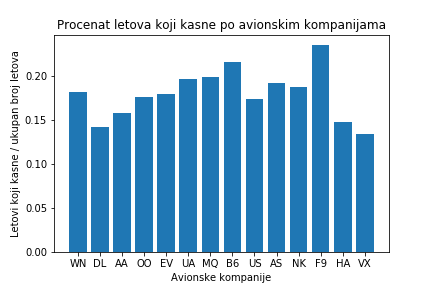
\includegraphics[scale=0.4]{slika1_n.png}
        \end{center}
    \end{figure}
\end{frame}


\begin{frame}{Podaci}
    \begin{itemize}
        \item podaci o letovima u SAD za 2015 godinu
        \item preko 5 miliona redova
        \item 30 atributa
        \begin{itemize}
                \item podaci o letovima (day, day of the
week, airline, flight number, tail number)
                \item podaci o polaznom i dolaznom aerodromu (origin airport, destination airport)
                \item informacije o poletanju (scheduled departure, departure time, departure delay, taxi-out, wheels-off)
                \item informacije o letu (scheduled time, elapsed time, air time, distance)
                \item informacije o dolasku (wheels-on,
taxi-in, scheduled arrival, arrival time, ar-
rival delay)
				\item dodatne informacije (air system delay, se-
curity delay, airline delay, late aircraft delay,
weather delay)
        \end{itemize}

    \end{itemize}
\end{frame}

\begin{frame}{Priprema podataka}
    \begin{itemize}
        \item 300 000 random redova
        \item indikator da li let kasni ili ne
        \item jednak broj letova koji su zakasnili i onih koji nisu
    \end{itemize}
\end{frame}

\begin{frame}{Primenjeni algoritmi}
    \begin{itemize}
        \item Logisticka regresija
        \item Potporni vektori
        \begin{itemize}
        	\item linerni
        	\item rbf kernel
        \end{itemize}
        \item Neuronske mreže
        \begin{itemize}
        	\item 3 sloja
        	\item prvi sloj 100 neurona, drugi 40
        	\item na prva dva sloja \emph{relu} aktivaciona funkcija, na posldenjem sigmoidna funkcija
        \end{itemize}
    \end{itemize}
\end{frame}

\begin{frame}{Problemi}
    \begin{itemize}
        \item traženje najboljih parametara za svm sa rbf kernelom
        \item neuronske merže za regresiju
        \item bolji razultati sa uzetih prvih 300 000 redova
    \end{itemize}
\end{frame}

\begin{frame}{Dobijeni rezultati}

\begin{tabular}{ |p{2cm}||p{2cm}|p{2cm}|p{2cm}|  }
 \hline
 \multicolumn{4}{|c|}{Mere kvaliteta} \\
 \hline
  & Tačnost &Odziv&F1 mera\\
 \hline
 Logistička regresija& 0.910    &0.889&  0.907\\
 Linearni svm&   0.909  & 0.889   &0.907\\
 Rbf  & 0.904& 0.883&  0.902\\
 Neuronska mreža    &0.929 & 0.886&  0.907\\
 \hline
\end{tabular}

\end{frame}


\begin{frame} 
	\begin{itemize}
		\item link ka aplikaciji
			\begin{itemize}
			\item https://github.com/anja-ivanisevic/ML\textunderscore projekat
			\end{itemize}
		\item link ka podacima
			\begin{itemize}
				\item https://www.kaggle.com/usdot/flight-delays/data
			\end{itemize}
		\item literatura
			\begin{itemize}
				\item http://cs229.stanford.edu/proj2017/final-reports/5243248.pdf
    			\item http://ml.matf.bg.ac.rs/readings/ml.pdf
			\end{itemize}
	\end{itemize}
\end{frame}


\begin{frame}{}
    \centering
    Hvala na pažnji!
\end{frame}


\end{document}
